% replace all text with your own text.
% in this template few examples are mention
\chapter{Methodology}
\label{ch:method} % Label for method chapter
Recognizing the need for early detection and management of cardiovascular conditions, we utilize machine learning algorithms to analyze patient data and predict the likelihood of heart disease. Our methodology encompasses data collection, preprocessing, feature extraction, model development, and evaluation, aiming to deliver a robust and effective predictive tool for doctors. By integrating innovative learning algorithms and conducting experiments, we aspire to contribute meaningful solutions and enhance patient outcomes in cardiovascular health.

\section{Algorithms Descriptions}
\subsection{Logistic Regression}
LR is a statistical method used for binary classification tasks. It models the probability of a binary outcome based on one or more predictor variables. In the context of heart disease prediction, LR can analyze patient parameters such as age, cholesterol levels, and blood pressure to estimate the likelihood of the presence of heart disease.

\subsection{Naïve Bayes}
NB is a probabilistic classifier based on Bayes' theorem with an assumption of independence between features. In heart disease prediction, Naïve Bayes can effectively analyze patient attributes and calculate the conditional probability of heart disease given the observed features. Its simplicity and computational efficiency make Naïve Bayes a popular choice for healthcare applications.

\subsection{Random Forest}
RF is an ensemble learning method that constructs a multitude of decision trees during training and outputs the mode of the classes (classification) or mean prediction (regression) of the individual trees. In heart disease prediction, Random Forest can analyze a large number of patient parameters and identify complex patterns associated with cardiovascular conditions.

\section{Implementations}
\subsection{Logistic Regression}
For LR implementation, we'll utilize the `LogisticRegression` class from the `sklearn.linear\_model` module. We'll preprocess the dataset, including handling missing values and scaling features, before fitting the model to the training data.
\subsection{Naïve Bayes}
For NB implementation, we'll use the `GaussianNB` class from the `sklearn.naive\_bayes` module. Similar to Logistic Regression, we'll preprocess the dataset and fit the model to the training data.
\subsection{Random Forest}
For RF implementation, we'll employ the `RandomForestClassifier` class from the `sklearn.ensemble` module. We'll preprocess the dataset and tune hyperparameters, such as the number of estimators and maximum depth, to optimize model performance.

\section{Experiments Design}
In our experimental approach to assess the predictive performance of each algorithm for heart disease, we'll begin by dividing our dataset into separate training and testing sets. This division ensures that the models are trained on a subset of the data and evaluated on an independent portion, enabling us to gauge their generalization capability. To further fortify the reliability of our findings, we'll employ cross-validation techniques. This involves iteratively partitioning the dataset into multiple subsets, training the models on different combinations, and validating them on the remaining data, thus providing a more comprehensive evaluation. Subsequently, we'll utilize a range of performance metrics, including accuracy, precision, recall, and F1-score, to quantify the algorithms' effectiveness. These metrics will allow us to discern not only the models' overall correctness but also their ability to precisely identify positive cases and recall them accurately. By meticulously analyzing these performance indicators, we aim to determine the most optimal approach for heart disease prediction, considering factors such as model interpretability and computational efficiency alongside predictive accuracy.

\section{Algorithms}
In our project, we implement three distinct machine learning algorithms—Logistic Regression, Random Forest, and Naive Bayes—to predict heart disease. Logistic Regression is a simple yet powerful algorithm used for binary classification tasks, where it models the probability of a binary outcome. Random Forest, on the other hand, is an ensemble learning method that constructs multiple decision trees and aggregates their predictions to improve accuracy. Naive Bayes is a probabilistic classifier based on Bayes' theorem, particularly effective for datasets with high dimensionality and strong feature independence assumptions. Each algorithm offers unique advantages and approaches in identifying patterns and making predictions, contributing to our comprehensive analysis of heart disease prediction.

\begin{algorithm}
    \caption{Logistic Regression}
    \label{algo:logistic_regression}
    \begin{algorithmic}[1]
        \Require{Training dataset $(X_{train}, Y_{train})$, Test dataset $X_{test}$}
        \Ensure{Predicted class labels for $X_{test}$}
        \Statex
        \Function{LogisticRegression}{$X_{train}, Y_{train}, X_{test}$}
        \State Initialize logistic regression classifier
        \State Standardize features: $X_{train} \gets \text{StandardScaler.fit\_transform}(X_{train})$
        \State Fit classifier to training data: $classifier.fit(X_{train}, Y_{train})$
        \State Standardize test features: $X_{test} \gets \text{StandardScaler.transform}(X_{test})$
        \State Predict probabilities for test data: $y_{prob} \gets classifier.predict\_proba(X_{test})$
        \State Convert probabilities to class labels: $y_{pred} \gets \text{threshold\_function}(y_{prob})$
        \State \Return $y_{pred}$
        \EndFunction
    \end{algorithmic}
\end{algorithm}

\begin{algorithm}
    \caption{Random Forest}
    \label{algo:random_forest}
    \begin{algorithmic}[1]
        \Require{Training dataset $(X_{train}, Y_{train})$, Test dataset $X_{test}$}
        \Ensure{Predicted class labels for $X_{test}$}
        \Statex
        \Function{RandomForest}{$X_{train}, Y_{train}, X_{test}$}
        \State Initialize random forest classifier with specified parameters
        \State Handle missing values: $X_{train}, X_{test} \gets \text{Imputer.fit\_transform}(X_{train}, X_{test})$
        \State Fit classifier to training data: $classifier.fit(X_{train}, Y_{train})$
        \State Predict class labels for test data: $y_{pred} \gets classifier.predict(X_{test})$
        \State \Return $y_{pred}$
        \EndFunction
    \end{algorithmic}
\end{algorithm}

\begin{algorithm}
    \caption{Naive Bayes}
    \label{algo:naive_bayes}
    \begin{algorithmic}[1]
        \Require{Training dataset $(X_{train}, Y_{train})$, Test dataset $X_{test}$}
        \Ensure{Predicted class labels for $X_{test}$}
        \Statex
        \Function{NaiveBayes}{$X_{train}, Y_{train}, X_{test}$}
        \State Initialize naive Bayes classifier
        \State Discretize continuous features: $X_{train}, X_{test} \gets \text{Binarizer.fit\_transform}(X_{train}, X_{test})$
        \State Fit classifier to training data: $classifier.fit(X_{train}, Y_{train})$
        \State Predict class labels for test data: $y_{pred} \gets classifier.predict(X_{test})$
        \State \Return $y_{pred}$
        \EndFunction
    \end{algorithmic}
\end{algorithm}


\begin{figure}
    \centering
    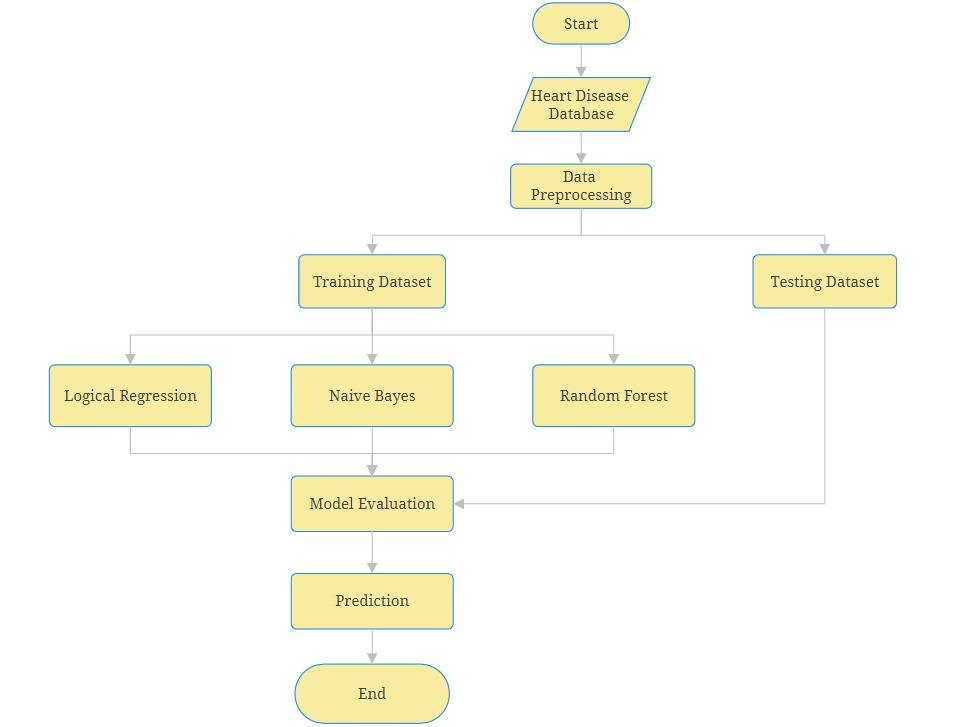
\includegraphics[width=1\linewidth]{figures/Flowchart.jpg}
    \caption{Flowchart of Heart Disease Prediction using LR, RF and NB}
    \label{fig:enter-label}
\end{figure}

\section{Example of code snippet  in \LaTeX}

Code Listing~\ref{list:python_code_ex} is a good example of including a code snippet in a report. While using code snippets, take care of the following:
\begin{itemize}
    \item do not paste your entire code (implementation) or everything you have coded. Add code snippets only. 
    \item The algorithm shown in Algorithm~\ref{algo:algo_example} is usually preferred over code snippets in a technical/scientific report. 
    \item Make sure the entire code snippet or algorithm stays on a single page and does not overflow to another page(s).  
\end{itemize}

Here are three examples of code snippets for three different languages (Python, Java, and CPP) illustrated in Listings~\ref{list:python_code_ex}, \ref{list:java_code_ex}, and \ref{list:cpp_code_ex} respectively.  

\begin{lstlisting}[language=Python, caption={Code snippet in \LaTeX ~and  this is a Python code example}, label=list:python_code_ex]
import numpy as np

x  = [0, 1, 2, 3, 4, 5] # assign values to an array
evenSum = evenSummation(x) # call a function

def evenSummation(x):
    evenSum = 0
    n = len(x)
    for i in range(n):
        if np.mod(x[i],2) == 0: # check if a number is even?
            evenSum = evenSum + x[i]
    return evenSum
\end{lstlisting}

Here we used  the ``\textbackslash clearpage'' command and forced-out the second listing example onto the next page. 
\clearpage  %
\begin{lstlisting}[language=Java, caption={Code snippet in \LaTeX ~and  this is a Java code example}, label=list:java_code_ex]
public class EvenSum{ 
    public static int evenSummation(int[] x){
        int evenSum = 0;
        int n = x.length;
        for(int i = 0; i < n; i++){
            if(x[i]%2 == 0){ // check if a number is even?
                evenSum = evenSum + x[i];
            }
        }
        return evenSum;     
    }
    public static void main(String[] args){ 
        int[] x  = {0, 1, 2, 3, 4, 5}; // assign values to an array
        int evenSum = evenSummation(x);
        System.out.println(evenSum);
    } 
} 
\end{lstlisting}


\begin{lstlisting}[language=C, caption={Code snippet in \LaTeX ~and  this is a C/C++ code example}, label=list:cpp_code_ex]
int evenSummation(int x[]){
    int evenSum = 0;
    int n = sizeof(x);
    for(int i = 0; i < n; i++){
        if(x[i]%2 == 0){ // check if a number is even?
            evenSum = evenSum + x[i];
    	}
    }
    return evenSum;     
}

int main(){
    int x[]  = {0, 1, 2, 3, 4, 5}; // assign values to an array
    int evenSum = evenSummation(x);
    cout<<evenSum;
    return 0;
}
\end{lstlisting}



\section{Example of in-text citation style}
\subsection{Example of the equations and illustrations placement and reference in the text}
Make sure whenever you refer to the equations, tables, figures, algorithms,  and listings for the first time, they also appear (placed) somewhere on the same page or in the following page(s). Always make sure to refer to the equations, tables and figures used in the report. Do not leave them without an \textbf{in-text citation}. You can refer to equations, tables and figures more them once.

\subsection{Example of the equations and illustrations style}
Write \textbf{Eq.} with an uppercase ``Eq`` for an equation before using an equation number with (\textbackslash eqref\{.\}). Use ``Table'' to refer to a table, ``Figure'' to refer to a figure, ``Algorithm'' to refer to an algorithm and ``Listing'' to refer to listings (code snippets). Note that, we do not use the articles ``a,'' ``an,'' and ``the'' before the words Eq., Figure, Table, and Listing, but you may use an article for referring the words figure, table, etc. in general.

For example, the sentence ``A report structure is shown in \textbf{the} Table~\ref{tab:gen_template}'' should be written as ``A report structure is shown \textbf{in} Table~\ref{tab:gen_template}.'' 
 

\section{Summary}
Write a summary of this chapter.

~\\[5em]
\noindent
{\huge\textbf{Note:}} In the case of \textbf{software engineering} project a Chapter ``\textbf{Testing and Validation}'' should precede the ``Results'' chapter. See Section~\ref{subsec:se_chpters} for report organization of such project. 

